\chapter{Conclusiones}
\label{chap:results}

\torev{Última revisión realizada el 25-06-2012}

El objetivo inicial del proyecto era, como se ha detallado a lo largo del documento, construir una herramienta capaz de transmitir musicalmente lo que se percibe de una imagen. Tras 9 meses de proceso de desarrollo, se puede afirmar que se ha desarrollado de forma satisfactoria una aplicación capaz de llevar a cabo dicho objetivo, así como el resto de requisitos (tanto funcionales como no funcionales) mostrados en la Sección~\ref{sec:requisitos}.\\



Para llevar a cabo la aplicación, ésta se ha dividido en dos módulos independientes que trabajan de forma secuencial: el módulo de análisis de imagen en primer lugar, y el módulo encargado de la composición musical en segundo; los cuales se pueden asemejar a la etapa de estimulación visual y a la etapa de estimulación auditiva, respectivamente. Esta distinción ha dado la posibilidad de estudiar y probar las etapas de forma independiente y así poder experimentar las diferentes formas de abordar la interpretación música-imagen. Cabe destacar que, dado que esta relación debe ser objetiva y no dependiente de consideraciones culturales o personales (por especificación del sistema), se ha elegido la sinestesia como método de asociación entre la percepción visual y la auditiva.\\


Por un lado, el módulo de análisis ha resultado ser capaz de transformar cualquier tipo de imagen de entrada en una representación propia del sistema de forma suficientemente fiel en un espacio de tiempo corto (segundos): dada una correcta configuración de parámetros por parte del usuario, las imágenes de grandes dimensiones pueden ser tratadas con menos nivel de detalle para aumentar su velocidad. Además, se puede cambiar la manera de reconocer formas alternando entre los distintos algoritmos de análisis, permitiendo al usuario experimentar con la forma en la que quiere que una imagen sea captada. La correcta elaboración de este módulo ha sido una pieza clave para el desarrollo del proyecto ya que, aunque no sea el objetivo principal del mismo, proporciona la entrada al módulo de composición y por tanto una pieza clave para el perfecto funcionamiento de la generación de música.\\

Por otro lado, el módulo de composición ha cumplido con las expectativas mencionadas a lo largo del documento, siendo capaz de componer piezas musicales completamente originales que, si bien no buscan propiedades como ser ``pegadizas'', en ningún momento son dejan de ser agradables al oído. Además, el módulo permite al usuario cambiar la forma de componer cada voz, así como los instrumentos con los que se interpretará cada una de ellas.\\

Con todo esto, la aplicación satisface la posibilidad de ser testeada por personas sinestésicas, de forma que éstas sean capaces de reconocer parcial o totalmente la similitud entre la imagen de entrada y la música generada. Con las diversas pruebas realizadas durante el desarrollo del proyecto, se ha determinado que la posibilidad de identificar la música creada a partir de las imágenes es factible, pero razonablemente limitada. Esto es debido a la cantidad de información que proporciona cada análisis de imagen, ya que sólo en las imágenes simples (con poca información) se puede anticipar la música generada. \color{blue}Por poner un ejemplo, una figura de cuatro vértices se asociará con cuatro notas. A cada figura interna dentro de ella se le asignará una melodía secundaría que sonará a la vez que la melódia de la figura padre. No hay que olvidar que, para añadir riqueza a la pieza musical, se añade una tercera voz (el bajo) y otra voz rítmica también basadas en las figuras presentes. Con todo esto, una figura de pocos vértices con unas pocas figuras dentro de ella tendrá asociada una pieza musical con cuatro voces tocando melodías distintas de una duración moderadamente corta a la vez. Por otro lado, una imagen analizada tiene del orden de un centenar de polígonos dentro de ella, cada uno de ellos con decenas de vértices. Puede imaginar el lector la complejidad que presentará la pieza musical generada, razón por la cual aumenta considerablemente la dificultad de compender el origen de las notas que ha compuesto el algoritmo en cada momento.\color{black}\\


\section{Usos de la aplicación}
\label{sec:usos}

Esta aplicación ha sido desarrollada teniendo en cuenta varios tipos de mercados (escenarios) y no sólo los pertenecientes al sector musical, ya que además de ellos se proponen otras alternativas. Es por ello que los usos para los cuales este sistema ha sido diseñado son:

\begin{itemize} 

\item\textbf{Ayuda a la composición:} Uno de los mayores problemas a la hora de componer es la búsqueda de inspiración para crear nuevas piezas musicales. Es por ello que un generador de música de esta índole, capaz de generar piezas originales y de un estilo razonablemente predecible (ya que depende de forma determinista de una imagen de entrada) es de gran utilidad en  este ámbito, siendo capaz de proporcionar ideas a los usuarios compositores. Con el objetivo de enfocar la aplicación a este aspecto, se ha establecido contacto con varios músicos quienes han mostrado su interés y admitido la posibilidad de usar la aplicación para tal fin. \color{blue} Durante sus experiencias, han preferido usar la aplicación con una gran variedad de imágenes, con la finalidad de abastecerse de piezas musicales variadas en lugar de intentar ver los diferentes efectos que puede tener el cambio de parámetros en una misma imagen, dado que el resultado sería una pieza musical similar a la pieza generada por primera vez. Sus opiniones han sido tremendamente positivas, apreciando la utilidad de dos aspectos de la aplicación: la creación de partituras, ya que sirve como base para componer una canción más complicada a partir de ella, y la reproducción de la música generada dentro del mismo entorno, gracias a la cual se puede comprobar rápidamente el resultado de una composición y se agiliza la realización de pruebas.\color{black}

\item\textbf{Composición visual:} \color{blue} En una rama puramente artística, la asociación de imagen-música proporcionada por esta aplicación puede servir como punto de partida de una corriente artística que consista en elaborar piezas gráficas con la intención de ser interpretadas como música por ésta o una aplicación similar.\color{black}


\item\textbf{Generación de música ambiente temática:} Como se ha establecido en la introducción de este documento, la generación musical desarrollada no pretende componer piezas musicales que sean capaces de ser el foco de atención del usuario durante su interpretación, sino que es su objetivo generar una música de ambiente capaz de sonar de fondo mientras el usuario realiza otra actividad. Dado que se une la percepción visual con la musical, es una forma más de realidad aumentada que puede servir como hilo musical de fondo en museos (con melodías asociadas a cuadros), anuncios (melodías asociadas al logo de la marca promocionada) o distintas situaciones cotidianas.

\item\textbf{Educación:} Tanto los niños pequeños como los discapacitados (con enfermedades como el autismo o similares) sienten una gran conexión con la música y están bastante atraídos por ella. Mediante el uso de esta aplicación pueden aprender a crear música de forma sencilla y además divertida, al mismo tiempo que entrena su percepción visual, desarrollando por tanto los dos sentidos simultáneamente. Se ha comentado esta idea a personas dentro del sector educativo que han mostrado interés en probar esta aplicación en cursos con alumnos más pequeños.

\end{itemize}

\section{Futuras ampliaciones}
\label{sec:ampliaciones}

Una vez desarrollada la aplicación, y siendo ésta completamente funcional, cabe plantearse las posibles ampliaciones que se podrían realizar sobre el sistema para incrementar su funcionalidad y usos. Muchas de ellas parten de la idea inicial del proyecto, con la intención de proporcionar robustez al sistema o mejorar su funcionalidad; otras buscan dar al sistema un nuevo enfoque de uso. Estas ampliaciones son:

\begin{itemize}

\item\textbf{Realización de nuevos y distintos algoritmos de composición:} Aunque los algoritmos desarrollados se basan todos en una idea común (la sinestesia), existen muchas maneras de interpretar una imagen estática como una pieza musical que evoluciona en el tiempo. El proyecto ha sido diseñado para poder añadir nuevos algoritmos
al código fuente de forma razonablemente sencilla. El proceso de desarrollo de estos algoritmos se basa intrínsecamente en el desarrollo y realización constante de pruebas, por lo que no existe una solución definitiva.\\

Para ello, se puede partir de ayuda externa para producir ideas (o bien búsqueda y lectura de investigaciones llevadas a cabo sobre estos aspectos de la composición, o bien contacto con compositores profesionales). Además, es necesaria en la elaboración de nuevos algoritmos un post-proceso de testeo de la cualidad de los mismos, ya que la calidad de las piezas musicales generadas por un algoritmo no se puede demostrar con completa seguridad hasta la finalización de la implementación de los algoritmos.

\item\textbf{Permitir la inclusión de nuevos algoritmos externos al código fuente.} Actualmente, la única manera de incluir nuevos algoritmos de composición o análisis es incluyéndolos en el código fuente de la aplicación. Una posible vía de desarrollo consistiría en dar la oportunidad al usuario de incluir nuevas formas de componer y analizar de forma externa, mediante nuevos módulos ejecutables o scripts que la aplicación sea capaz de lanzar.\\

\item\textbf{Expandir el formato de representación de imágenes}, de forma que sea capaz de almacenar más información sobre la imagen. La aplicación desarrollada sólo es capaz de representar internamente polígonos y sus posiciones y colores; pero hay mucha más información dentro de una imagen que nos puede ser útil:

	\begin{itemize}
	
		\item\textit{Reconocimiento de simetrías:} una imagen puede tener diferentes tipos de simetrías entre los objetos/colores que la forman. Información de este tipo puede servir de base a nuevos algoritmos de composición para que realicen melodías que repitan patrones o segmentos en función de las simetrías encontradas.
		
		\item\textit{Reconocimiento de composiciones:} no es poco común que las figuras de una imagen estén dispuestas siguiendo formas geométricas básicas (círculos o triángulos, por poner dos ejemplos). Un ejemplo bastante famoso se puede observar en la Figura~\ref{fig:composition}, donde se muestra la imagen de entrada a la izquierda y la composición que se pretende reconocer a la derecha. Imágenes con una disposición geométrica de figuras muy acentuada puede producir composiciones musicales cuya organización global sea equivalente a esta geometría detectada.\\
			
			\begin{figure}[!htbp]
			\centering
			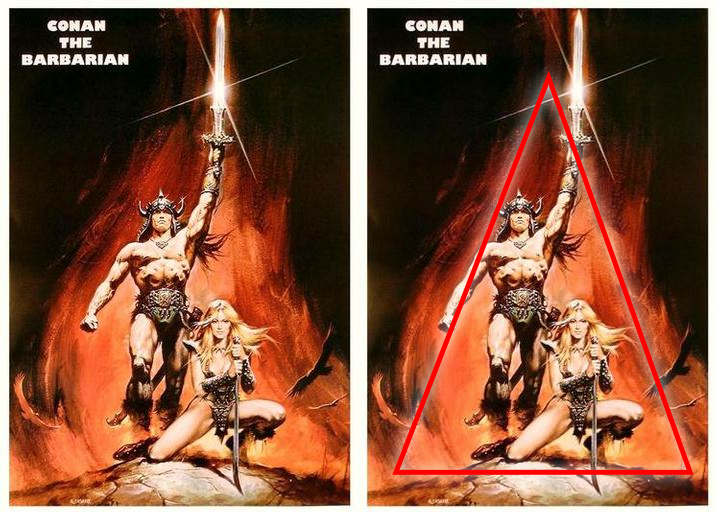
\includegraphics[scale=0.40]{graphics/composition2.png}
			\caption{Ejemplo de reconocimiento de una composición triangular.}
			\label{fig:composition}
			\end{figure}
		
		\item\textit{Reconocimiento de estructuras fractales:}
\color{blue}existen actualmente compositores algorítmicos que toman como entrada los parámetros de una estructura fractal para generar piezas musicales acordes a ella. De forma más ambiciosa, el proceso de análisis de este sistema podría distinguir aquellos casos en los que las figuras de una imagen forman entre sí estructuras fractales, es decir, donde formas básicas se repiten en diferentes dimensiones, como se da en la Figura~\ref{fig:fractal}. Posteriormente, esta información se pasaría a un compositor que tenga en cuenta estas estructuras.\color{black}
		
			\begin{figure}[!htbp]
			\centering
			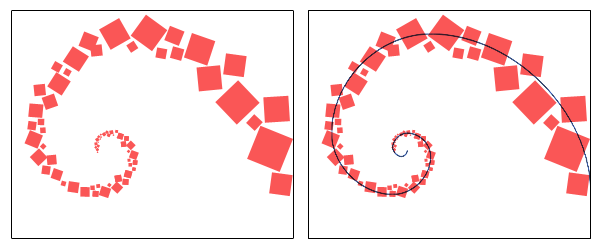
\includegraphics[scale=0.47]{graphics/fractal.png}
			\caption{Ejemplo de reconocimiento de una estructura fractal.}
			\label{fig:fractal}
			\end{figure}

		\item\textit{Ampliación de descripción del color de una figura:} la aplicación actual, con el objetivo de simplificar el proceso de análisis, sólo reconoce un color para cada figura reconocida. Sin embargo, la figura puede experimentar dentro de ella una variación de colores (aunque sea dentro de pequeños rangos), hecho que el sistema simplifica calculando el color medio. Esta ampliación consistiría en investigar una manera de detectar esa variación interna de color de forma que se consiga una representación más fiel de la figura.
	\end{itemize}
	
\item\textbf{Portar la aplicación a sistemas Apple.} Con esto se conseguiría expandir el número de posibles usuarios de la aplicación. Dado que las máquinas con sistema operativo de Apple funcionan con UNIX como base, esta ampliación puede resultar muy sencilla si se parte de la versión para Linux de la aplicación.

\item\textbf{Portar la aplicación a sistemas móviles.} Una de las ideas iniciales que se debatieron antes de comenzar el desarrollo de la aplicación fue la de implementar el sistema como una aplicación móvil. Sin embargo, al realizar el estudio de alcance del proyecto y el tiempo de desarrollo del mismo, se desechó la idea. Sin embargo, una aplicación de esta índole puede alcanzar un gran éxito en estos dispositivos ya que las cámaras integradas de los mismos proporcionan una entrada gráfica fácil y sencilla, lo cual sumado a la facilidad de uso del sistema, proporcionan a la aplicación un gran atractivo.\\ 

El sistema se ha diseñado para facilitar la implementación de dicha ampliación, eligiendo librerías disponibles tanto en sistemas operativos de ordenadores personales como de dispositivos móviles (ver Sección~\ref{chap:techs}).\\

\end{itemize}


\section{Seguimiento del proyecto}

La aplicación, para cada una de las plataformas que ha sido desarrollada, se puede descargar desde aquí:

\begin{center}
http://code.google.com/p/muphic/downloads/list
\end{center}

Algunas piezas musicales compuestas a partir de imágenes por el software desarrollado están disponibles en este canal de \emph{youtube}:

\begin{center}
http://www.youtube.com/user/mrmuphic
\end{center}

Con el tiempo se irán añadiendo más resultados de las diferentes composiciones relevantes o especiales que se vean convenientes.\\

Para contactar con el grupo de proyecto se puede hacer a través de la siguiente dirección:

\begin{center}
	imagebasedcomposing@gmail.com
\end{center}